\documentclass[11pt,a4paper,landscape]{article}
\usepackage[utf8]{inputenc}
\usepackage[english]{babel}
\usepackage{amsmath}
\usepackage{cite}
\usepackage{amsfonts}
\usepackage{amssymb}
\usepackage{makeidx}
\usepackage{graphicx}
\usepackage{tikz}
\author{jacmalm@kth.se}
\title{DD2343 Assignment 1}
\begin{document}

\maketitle
\newpage
\section{Principal Component Analysis}

\subsection{Explain why data-centering is required before performing PCA.  What might happen if we perform PCA on non-centered data?}

The underlying assumption of PCA is that our observed variables \textbf{Y} have gone through a linear transformation.


\section{Multidimensional Scaling and Isomap}

\subsection{Argue that the process to obtain the neighbourhood graph G in the Isomap method may yield a disconnected graph.  Provide an example.  Explain why this is problematic.}

The Isomap algorithm works similarly to MDS in that it relies on computing a Gram matrix S from a distance matrix D.However,dissimilarly to MDS,this distance matrix is not made up of euclidean distances. Instead, the distances are approximations of the shortest path from point A to point B where the path is restricted to the theoretical manifold our data distribution makes up. Computing the shape of this manifold as well as the length of the path through the manifold from point A to B is infeasible. An approximation of the manifold can be created by drawing a neighbourhood graph G. This neighbourhood graph G is created one of two ways. Either by joining each point to its K nearest neighbours, where a point A is considered closer to point B than to C if the euclidean distance between A-B is smaller than A-C.  Alternatively the neighbourhood graph can be constructed by choosing to join a point A to all of its neighbours that lie within a certain distance \textit{d}.

To demonstrate how this process can lead to a disconnected graph,  assume we have the following nodes located at given coordinates.

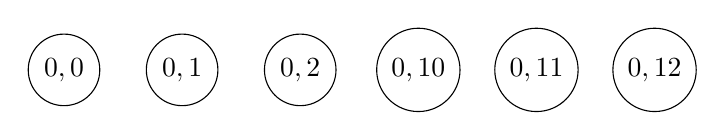
\begin{tikzpicture}[node distance=15mm, main/.style = {draw, circle}] 
\node[main] (1) {$0,0$}; 
\node[main] (2)[right of = 1] {$0,1$}; 
\node[main] (3)[right of = 2] {$0,2$}; 
\node[main] (4)[right of = 3] {$0,10$}; 
\node[main] (5)[right of = 4] {$0,11$}; 
\node[main] (6)[right of = 5] {$0,12$}; 

\end{tikzpicture}

If we go by the k-nearest neighbour approach and set k=2, or go by max euclidean distance between nodes and set \textit{d} to smaller than 8, our resulting graph will be disconnected.

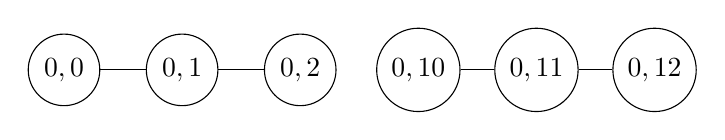
\begin{tikzpicture}[node distance=15mm, main/.style = {draw, circle}] 
\node[main] (1) {$0,0$}; 
\node[main] (2)[right of = 1] {$0,1$}; 
\node[main] (3)[right of = 2] {$0,2$}; 
\node[main] (4)[right of = 3] {$0,10$}; 
\node[main] (5)[right of = 4] {$0,11$}; 
\node[main] (6)[right of = 5] {$0,12$}; 
\draw(1) -- (2);
\draw(2) -- (3);
\draw(4) -- (5);
\draw(5) -- (6);
\end{tikzpicture}

According to the Isomap algorithm, when we compute the distance matrix, the entry between point A and point B will be the summation of the distances between all nodes that lie along the shortest path between A and B through the neighbourhood graph G constructed in the previous step. If this is a disconnected graph, the distance between any point A to any point B where A and B are members of different disjoint subsets in G will be infinite, or undefined. In either of these cases the spectral decomposition of the Gram matrix corresponding to the distance matrix will be undefined and the Isomap algorithm will fail.

\cite{stackexchange}

\bibliography{mybib}
\bibliographystyle{plain}
\end{document}